\documentclass[18pt]{beamer}
\usetheme{Madrid}

\usepackage{graphics}


\newcommand{\centeredlargetext}[3]{
{
\setbeamertemplate{navigation symbols}{}
\setbeamercolor{background canvas}{bg={#1}}
\color{#2}
\begin{frame}[plain]
\fontsize{36pt}{36pt}\selectfont
\center
\begin{center}
{#3}
\end{center}
\end{frame}
}}

\newcommand{\centeredhugetext}[3]{
{
\setbeamertemplate{navigation symbols}{}
\setbeamercolor{background canvas}{bg={#1}}
\fontsize{72pt}{72pt}\selectfont
\color{#2}
\begin{frame}[plain]
\center
\begin{center}
{#3}
\end{center}
\end{frame}
}}


\begin{document}

\title[ITKv4]{ITKv4 - The Next Generation}
\subtitle[ITKv4]{What is new in ITKv4}
\institute[Insight Software Consortium]{Insight Software Consortium}
\date[June 2011]{June 2011}

\begin{frame}
\titlepage
\end{frame}


{
\setbeamertemplate{navigation symbols}{}
\begin{frame}[plain]
\center
\begin{center}
This presentation is copyrighted by\\
The \textbf{Insight Software Consortium}\\
\bigskip
distributed under the\\
\textbf{Creative Commons by Attribution License 3.0}\\
\url{http://creativecommons.org/licenses/by/3.0}\\
\end{center}
\end{frame}
}


\begin{frame}
  \tableofcontents
\end{frame}


\centeredlargetext{white}{black}{
ITKv4
}


\section{Introduction}


\centeredlargetext{white}{black}{
Apache 2.0 License
}


\centeredlargetext{white}{black}{
New Software Process
}

\begin{frame}
\frametitle{Software Process}
\begin{itemize}
\item Git
\pause
\item Gerrit
\pause
\item cdash@home
\end{itemize}
\end{frame}

\centeredlargetext{white}{black}{
Modularization
}

\begin{frame}
\frametitle{Modularization}
\begin{itemize}
\item 98 Modules
\pause
\item Groups
\pause
\item External Modules
\end{itemize}
\end{frame}


\begin{frame}[fragile]
\frametitle{Modules Size}
\begin{center}
  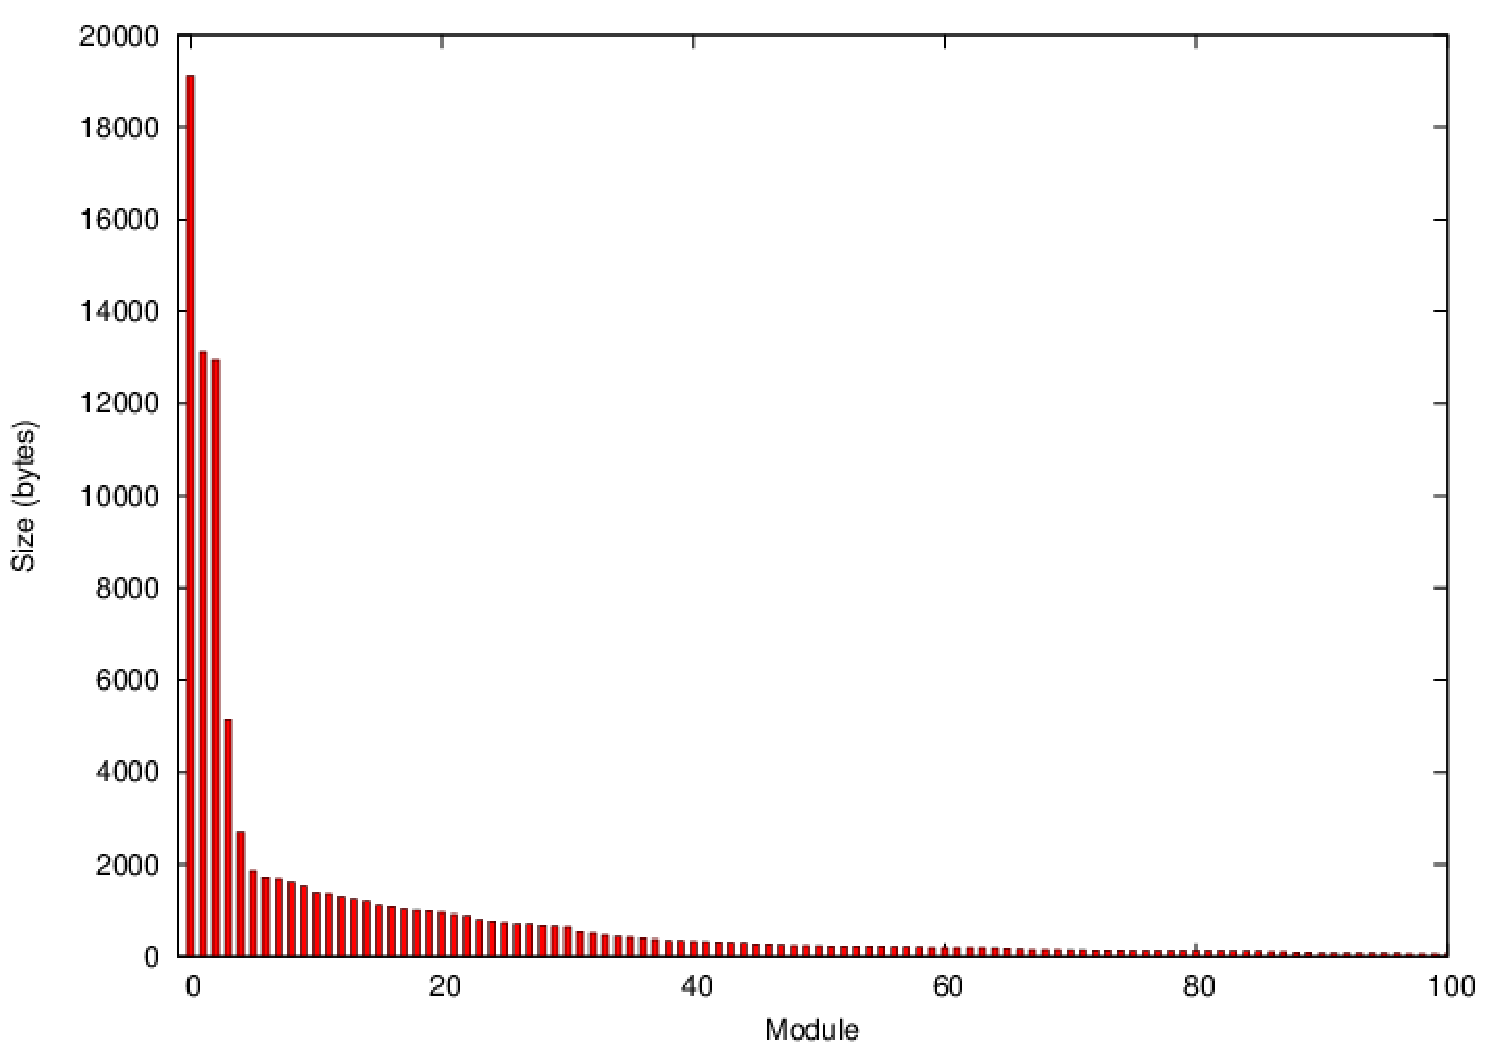
\includegraphics[width=0.5\paperwidth]{moduleSizePlot.pdf}
\end{center}
\end{frame}


\centeredlargetext{white}{black}{
Statistics Framework
}


\centeredlargetext{white}{black}{
FEM Refactoring
}

\begin{frame}
\frametitle{FEM Refactoring}
\begin{itemize}
\item Code Clean up
\pause
\item Removed subversive pointers
\end{itemize}
\end{frame}


\centeredlargetext{white}{black}{
Level Sets Refactoring
}

\begin{frame}
\frametitle{Level Sets Refactoring}
\begin{itemize}
\item Generalization for Images and Meshes
\pause
\item Modular Terms
\end{itemize}
\end{frame}


\centeredlargetext{white}{black}{
Image Registration Refactoring
}

\begin{frame}
\frametitle{Image Registration Refactoring}
\begin{itemize}
\item Composite Transform
\pause
\item Symmetric Registration
\pause
\item Transforms IO
\end{itemize}
\end{frame}


\centeredlargetext{white}{black}{
GPU
}


\begin{frame}
\frametitle{Image Registration Refactoring}
\begin{itemize}
\item Composite Transform
\pause
\item Symmetric Registration
\pause
\item Transforms IO
\end{itemize}
\end{frame}


\centeredlargetext{white}{black}{
SimpleITK
}


\begin{frame}
\frametitle{New Fields}
\begin{itemize}
\item Microscopy
\pause
\item Video
\pause
\item Remote Sensing
\end{itemize}
\end{frame}


\end{document}
